%%%%%%%%%%%%%%%%%%%%%%%%%%%%%%%%%%%%%%%%%%%%%%%%%%%%%%%%%%%%%%%%%%%%%%%%
% Plantilla TFG/TFM
% Escuela Politécnica Superior de la Universidad de Alicante
% Realizado por: Jose Manuel Requena Plens
% Contacto: info@jmrplens.com / Telegram:@jmrplens
%%%%%%%%%%%%%%%%%%%%%%%%%%%%%%%%%%%%%%%%%%%%%%%%%%%%%%%%%%%%%%%%%%%%%%%%

\chapter{Introduction}

This chapter will introduce the reader to the context of this project. It will
begin by providing a brief overview of the problem at hand, followed by a
description of the motivation behind this work. Finally, it will conclude with
a summary of the contents of the rest of the document.

\section{Motivation and context}

Obesity represents a pressing global public health concern, affecting a
significant segment of the population. \todo{why obesity is bad}.

Tech4Diet is an investigation project that aims to study how obesity treatments
affect morfological changes in the human body. \todo{more about tech4diet}

In a previous initiative, \todo{link} Tech4Diet developed a system enabling
patients undergoing weight loss treatment to visualize 3D scans of their bodies
throughout their weight loss journey~\cite{Azorin-Lopez2020}.

During the treatment, the patient's body is captured using an RGBD camera, the
Intel RealSense D435. The 3D model of the human body is shown during the
different sessions using a virtual reality headset. This innovative approach
aimed to boost motivation and increase treatment plan adherence.

\begin{figure}
	\centering
	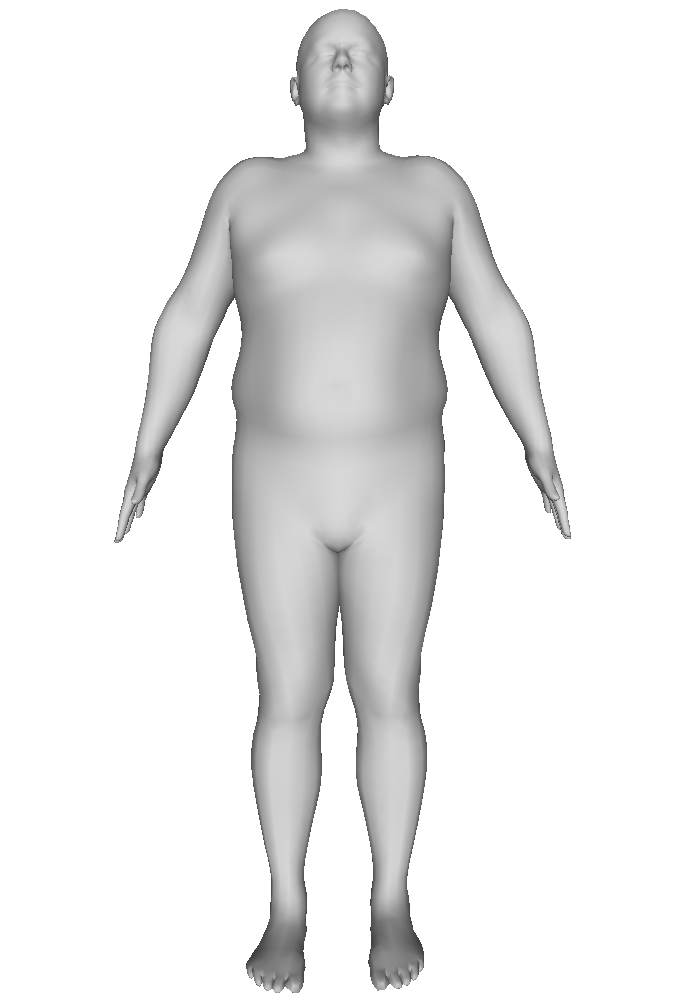
\includegraphics[width=75pt]{files/patient_8/2_cropped}
	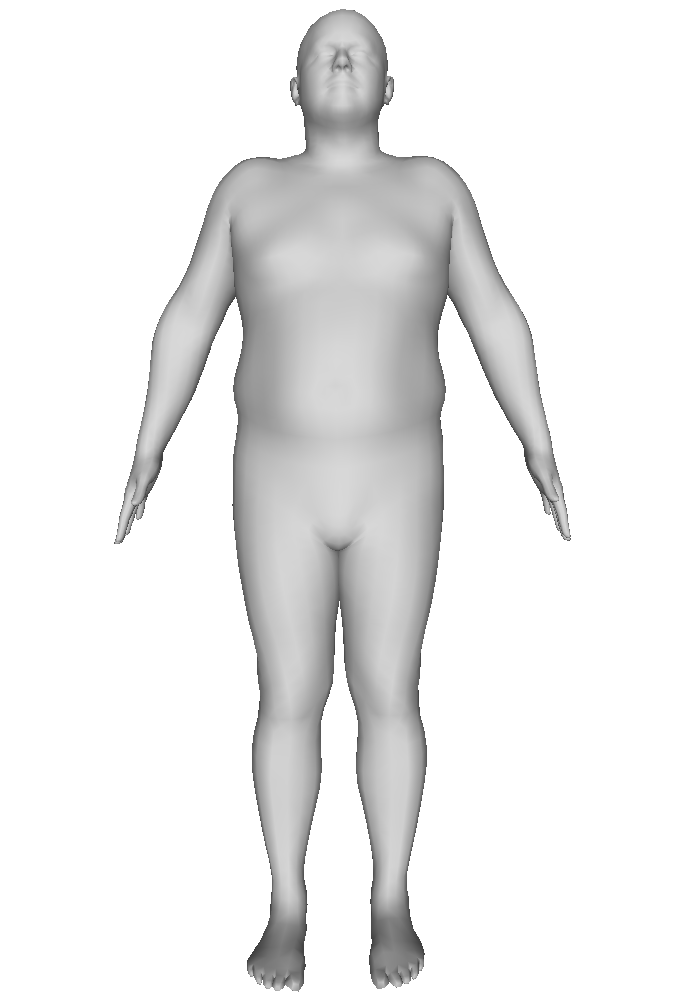
\includegraphics[width=75pt]{files/patient_8/3_cropped}
	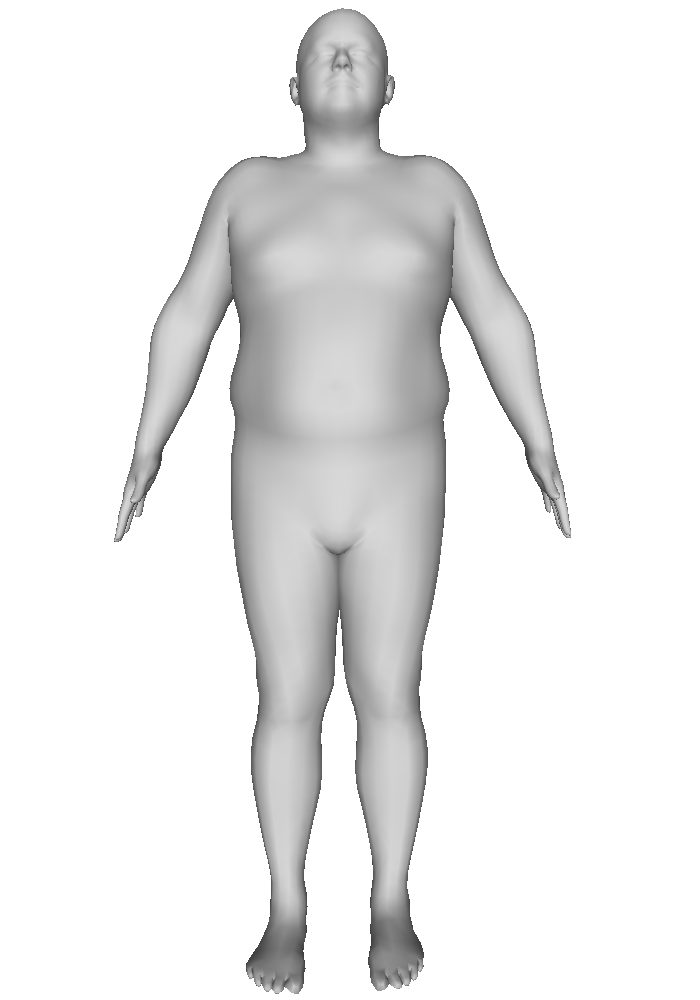
\includegraphics[width=75pt]{files/patient_8/4_cropped}
	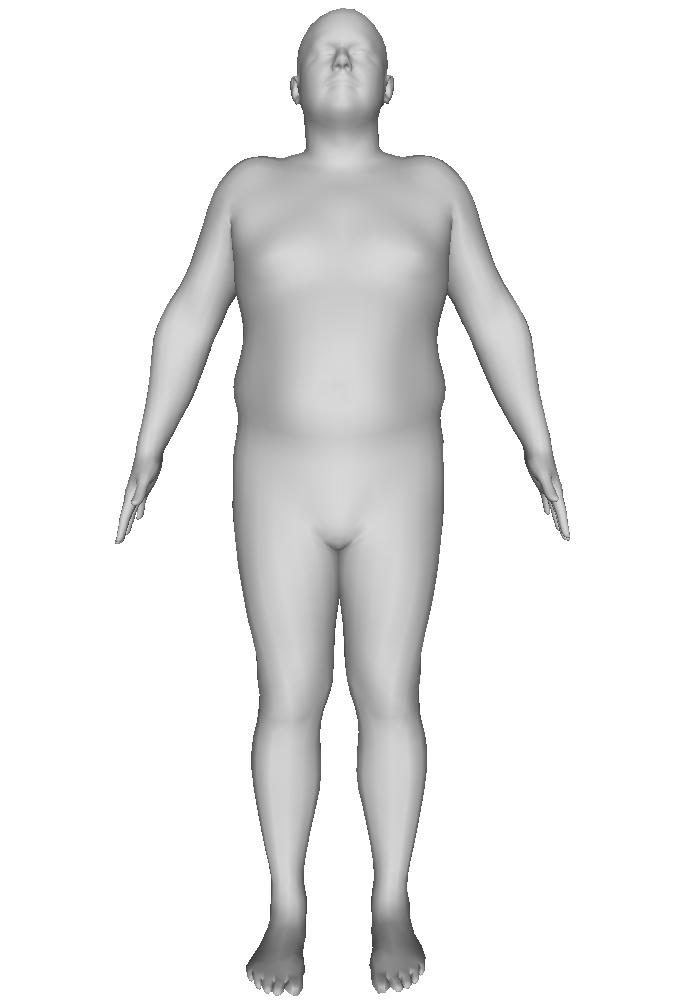
\includegraphics[width=75pt]{files/patient_8/5_cropped}
	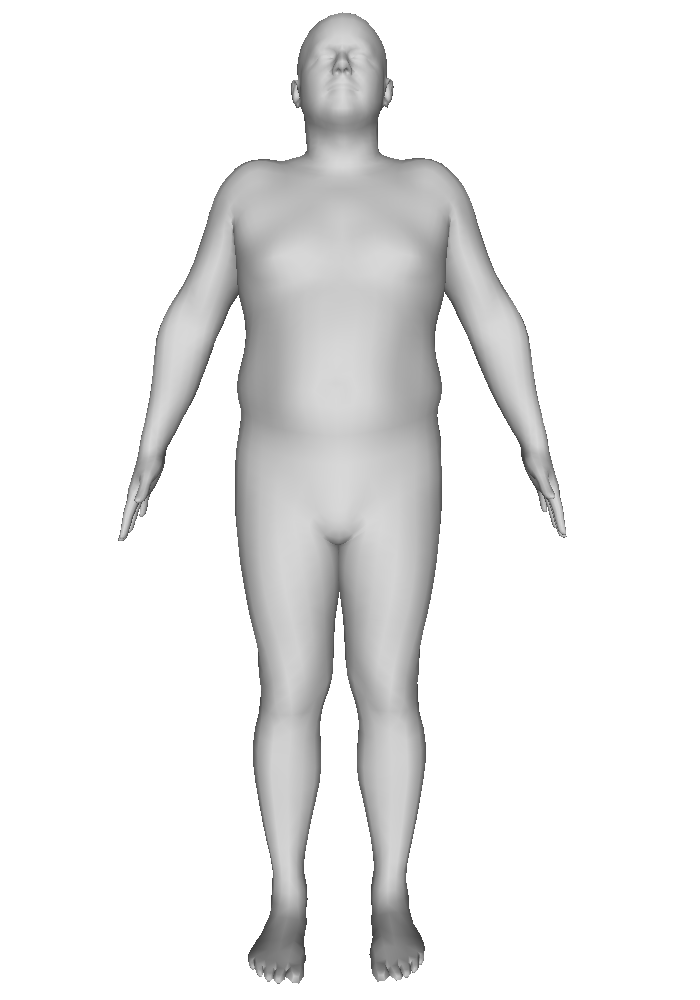
\includegraphics[width=75pt]{files/patient_8/6_cropped}
	\caption{3D model reconstruction of a patient's body at different stages of a weight loss
		treatment. There is around a month between each scan, and a total
		weight loss of 3.8 kg.}
\end{figure}

Besides body scans, the study also collected other medical data, including
variables such as weight, localized fat and muscle mass, activity levels and
other psychological factors.

Subsequently, we wondered if it would be feasible to utilize the datasets
acquired in this prior study to formulate a predictive model. This model would
project anticipated changes in a person's body undergoing weight loss treatment
before the treatment concludes, further bolstering adherence to the treatment
regimen.

The present work explores the development of such a model. This includes
analyzing data from the earlier study, reviewing existing techniques in human
body model representation, encoding patient data using the chosen
representation, devising a neural network architecture for predicting patient
body changes, training and evaluating the model and finally, generating 3D
meshes of the predicted body changes.

We will expand on the details of this process in the following chapters.
Chapter \nameref{data} will delve into the data collected during the previous
study, and how we processed it to prepare it for use in our model, as well as
how we encoded the human body scans. Afterwards, chapter \nameref{nn} will go
over the neural network architecture we devised for this project, as well as
the training process and the results obtained. Finally, chapter
\nameref{results} will discuss the results of our model, and chapter
\nameref{conclusion} will conclude the document with a summary of the work done
and possible future lines of research.

\section{Background}

As previously mentioned, this section will provide a brief overview of the
\gls{sota} in the field of human body representation and generative neural
network architectures. We were able to use what we learned from the research on
3D human body models to write and submit a paper to the \gls{iwann} 2023
conference. \todo{link}

\subsection{3D human body representation}

The field of 3D human body recovery has seen a significant advancement with the
development of parametric models. These methods use a set of parameters to
represent body shape and pose and are widely used for reconstructing 3D human
body. These methods have different features, with some focusing on body
deformations, others on shape and pose optimization, and others on the
separation of body shape into identity-specific and pose-dependent components,
among other things. The advancements in the field have led to improved accuracy
and stability in representing human body shapes and poses. On the other hand,
in recent years various generative methods have been developed to generate 3D
models of the human body. Variational Autoencoder (VAEs) and Generative
Adversarial Networks (GANs) are two commonly used types of neural networks for
this purpose. These methods can generate 3D human body models by learning the
distribution of the data. There are many areas that can make use of these
models. Some of the most significant applications include:

\begin{itemize}
	\item Medicine: Human body models are valuable in the study of
	      anatomy~\cite{https://doi.org/10.1002/ase.1718} and for patient monitoring.
	\item Film industry: Human body models can be used to capture motion data and render
	      high-quality CGI humans.
	\item Video game industry: Human body models can be used to create realistic
	      animations and interactions between characters\cite{Starke2021}.
	\item Extended reality: Human body models can be used to capture user input in
	      virtual reality as well as rendering realistic characters.
	\item Clothing: These models can be used for fitting virtual
	      clothes\cite{apeagyei2010application} and creating realistic images of clothing
	      products.
\end{itemize}

A straightforward approach to categorize human body representations is to
classify based on the required input type and the generated output.

Regarding input, representations fall into three categories:

\begin{itemize}
	\item 2D input: These representations utilize 2D images or videos as input.
	      Some models may also process images from varying angles. The flexibility
	      of these models is beneficial as they do not necessitate specific hardware
	      to capture the input data.
	\item 3D input: Typically, these models require 3D point clouds as input data.
	\item Parametric models: These models demand a set of parameters describing the body.
	      Some models categorize these parameters into body shape and body pose. This
	      form of representation is highly intriguing for machine learning applications
	      due to the significant reduction in input data dimensionality. This factor
	      permits the training of a neural network with fewer samples. However, it
	      necessitates a model capable of generating parameters from the input data.
\end{itemize}

Some of the most common 3D output types are:

\begin{itemize}
	\item 3D meshes: These models create a 3D mesh of the object.
	\item 3D voxel: These models produce a 3D voxel grid of the object.
	      However, this approach is not widespread as it is generally not
	      beneficial for most applications.
	\item \gls{nerf}: This novel 3D representation directly renders the object
	      from a specific viewpoint. While this allows for the generation of
	      highly realistic images, it proves less beneficial for applications
	      requiring a true 3D representation of the object.
\end{itemize}

\subsubsection{Generation}

When it comes to generating 3D human models, we distinguish two main
approaches. The first approach is to use a general purpose generator system and
guide it to generate human models. The second approach is to use a generator
that has been specifically designed to generate human models from the start.

\paragraph{Human specific}

SiCloPe \cite{SiCloPe} models clothed human bodies using deep generative
models. It can reconstruct a complete and textured 3D model of a person wearing
clothes from a single input picture. It uses a silhouette-based representation
that combines 2D silhouettes and 3D joints of a body pose to describe the
complex shape variations of clothed people. It synthesizes consistent
silhouettes and feeds them into a deep visual hull algorithm for 3D shape
prediction and uses a conditional generative adversarial network to infer the
texture of the subject's back view.

PIFu \cite{PIFu} is a highly effective implicit representation that locally
aligns pixels of 2D images with their corresponding 3D object. The method can
infer 3D surface and texture from a single image or multiple input images. It
can handle intricate shapes and their variations and deformations, and can
produce high-resolution surfaces including largely unseen regions such as the
back of a person. It extends naturally to arbitrary number of views and is
memory efficient, spatially aligned with the input image and can handle
arbitrary topology. PIFuHD \cite{PIFuHD} builds on top of PIFu with an
additional module and applies it to the task of human digitalization.

Tex2Shape \cite{Tex2Shape} is a simple method to infer detailed full human body
shape from a single photograph. It turns shape regression into an aligned
image-to-image translation problem and estimates detailed normal and vector
displacement maps from partial texture maps of the visible region. The results
feature details even on parts that are occluded in the input image and the
model generalizes well to real-world photographs.

HumanMeshNet \cite{HumanMeshNet} regresses a template mesh's vertices and
receives regularization from 3D skeletal locations in a multi-branch,
multi-task framework. It focuses on implicitly learning the mesh representation
and is a novel model for 3D human body reconstruction from a monocular image.

DeepHuman \cite{DeepHuman} is image-guided 3D human reconstruction network that
leverages a dense semantic representation and fuses different scales of image
features into the 3D space. The visible surface details are refined through a
normal refinement network. The method outperforms state-of-the-art approaches
in 3D human model estimation from a single image.

HumanGen \cite{humangen} is a 3D human generation scheme with detailed geometry
and 360° realistic free-view rendering. The scheme marries the 3D human
generation with various priors from the 2D generator and 3D reconstructor of
humans through the design of an "anchor image." The authors adopt a pronged
design to disentangle the generation of geometry and appearance and use an
anchor image to adapt a 3D reconstructor for fine-grained details synthesis and
propose a two-stage generation scheme for geometry and appearance.

HumanNeRF \cite{humannerf} describes a neural representation for high-fidelity
free-view synthesis of dynamic humans. It uses an aggregated pixel-alignment
feature with a pose embedded non-rigid deformation field and raw HumanNeRF can
already produce reasonable rendering on sparse video inputs. The approach is
improved with in-hour scene-specific fine-tuning and appearance blending. The
authors show that this approach is effective in synthesizing photorealistic
free-view humans with sparse camera view inputs.

\paragraph{General}

The CoCosNet \cite{CoCosNet} (and CoCosNet v2 \cite{CoCosNet2}) paper
introduces full-resolution correspondence learning for cross-domain image
translation. It uses a hierarchical strategy that employs the correspondence
from coarse to fine levels and utilizes the ConvGRU module to refine the
current correspondence. The result is a highly efficient and effective approach
for exemplar-based image translation that outperforms state-of-the-art
literature.

\subsubsection{Generative neural networks}

\section{Objectives}\label{objectives}

\begin{itemize}
	\item \strong{Objective 1} Study the state of the art in human body representation and
	      generation. \subitem Review the literature on human body representation and
	      generation. \subitem Analyze the advantages and disadvantages of the different
	      approaches. \subitem Select the most suitable approach for the project.
	\item \strong{Objective 2} Analyze and process the data to be used in the project. \subitem
	      Explore the data and its characteristics. \subitem Preprocess the data to be
	      used in the project, identifying and solving any issues that may arise.
	      \subitem Study what data augmentation techniques can be applied to the data.
	\item \strong{Objective 3} Design and implement a neural network that can understand human
	      bodies and train it to predict shape changes in time. \subitem Study the
	      different neural network architectures that can be used in a time series
	      prediction problem. \subitem Design a neural network architecture that can be
	      used to generate future human body shapes. \subitem Implement the neural
	      network architecture. \subitem Train the neural network. \subitem Evaluate the
	      predictions made by the neural network.
	\item \strong{Objective 4} Evaluate the results. \subitem Generate predicted human body
	      shapes for a set of input data. \subitem Evaluate the predictions.
\end{itemize}

